\documentclass[12pt,a4paper]{report}
\usepackage[a4paper,width=150mm,top=25mm,bottom=25mm,bindingoffset=6mm]{geometry}
\usepackage[utf8]{inputenc}
\usepackage[portuguese]{babel}
\usepackage[T1]{fontenc}
\usepackage{amsmath}
\usepackage{amsfonts}
\usepackage{amssymb}
\usepackage{blindtext}
\usepackage{indentfirst}

\usepackage{tikz}
\usetikzlibrary{arrows}
\usepackage{verbatim}

\usepackage{graphicx}
\graphicspath{{images/}}

\begin{document}
\begin{titlepage}
	\begin{center}
		\vspace*{1cm}

		\Huge
		\textbf{Relatório de Sinais e Sistemas}\\
		\Large
		\textbf{2017.2}

		\vspace{0.5cm}
		\Large
		Trabalho 01 - Caderno de Exercícios

		\vspace{1.5cm}

		
\includegraphics[scale=0.8]{pucrio}

		\vspace{1.5cm}

		\normalsize
		\textbf{Fernando Homem da Costa - 1211971}\\
		\textbf{Pedro Escalfoni - 1321234}

		\vfill

		\Large
		Departamento de Elétrica\\
		Pontifícia Universidade Católica do Rio de Janeiro\\
		ENG1400 - Sinais e Sistemas\\
		\today

	\end{center}
\end{titlepage}

%\newpage
\tableofcontents
\newpage

\section{Introdução}
\addcontentsline{toc}{section}{Introdução}



\section{Questão 1}
\addcontentsline{toc}{section}{Questão 1}
Essa questão aborda conceitos básicos sobre construção de sinais e suas representação em um domínio específico. Sobre os sinais dessa questão, podemos afirmar que eles são discretos, ou seja, possuem a sua variável independente "n" pertencente ao domínio do tempo discreto, onde "n" $\in$  $\mathbb{Z}$ . Além disso, propõe que os alunos possam conhecer as representações gráficas de sinais básicos, como, impulso unitário, degrau unitário, rampa unitária e a exponencial, considerando o intervalo exigido.

	\subsection{Letra (A)}
	\addcontentsline{toc}{section}{Letra (A)}
	 Podemos analisar pelos gráficos plotados pela função \textbf{stem()} cada um dos sinais discretos. Há superposição de sinais, logo, fizemos um gráfico para cada sinal e no final disponibilizamos todos em uma única janela grafica.
	 \begin{figure}[!ht]
		\centering
		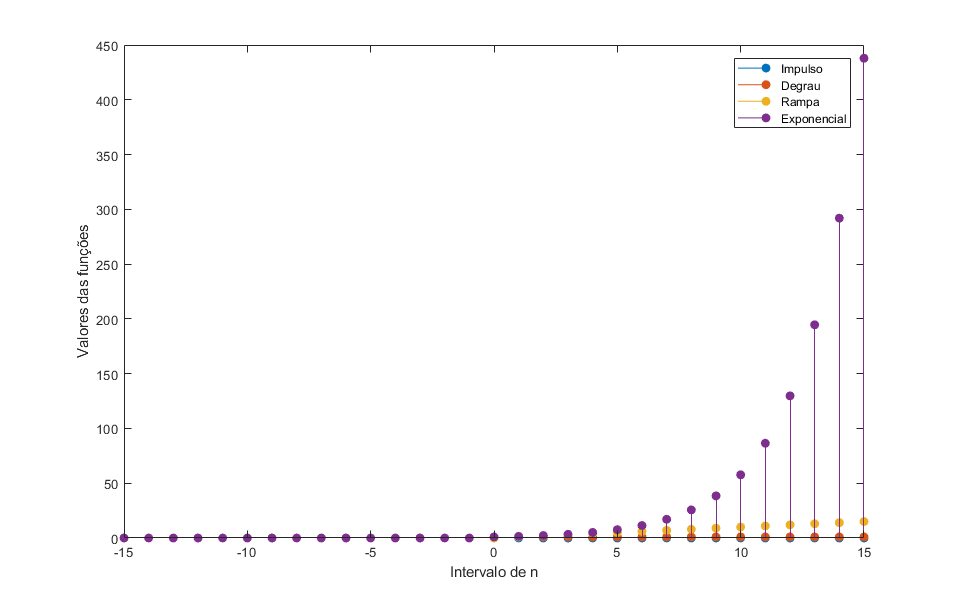
\includegraphics[scale=0.5]{1a-Tudo}
		\caption{Gráfico - Tudo}
	\end{figure}
 	Vemos que no sinal impulso unitario <latex dirac> para k(ou n, nao sei) != 0, os valores são zeros e em k = 0, impulso tem o valor unitario  <latex definicao dirac>. [insira janela grafica impulso aqui]
 	Para o degrau, temos que para k < 0; o sinal vale 0 e para k >= 0, o sinal vale 1, lembrando que o degrau unitário é a integral do inpulso unitario (kroenecker fernando! nao dirac) <latex kroenecker>. [insira janela grafica degrau aqui]
	Para a rampa, que é a integral do degrau, temos que para t < 0, o sinal vale 0 e para t >= 0; o sinal vale t <latex rampa>. [insira janela grafica rampa aqui]
	A exponencial vale 0 para t < 0 e e^a*t para t >=0 <latex exponencial>. [insira janela grafica exponencial aqui]
			\begin{figure}[!ht]
				\centering
				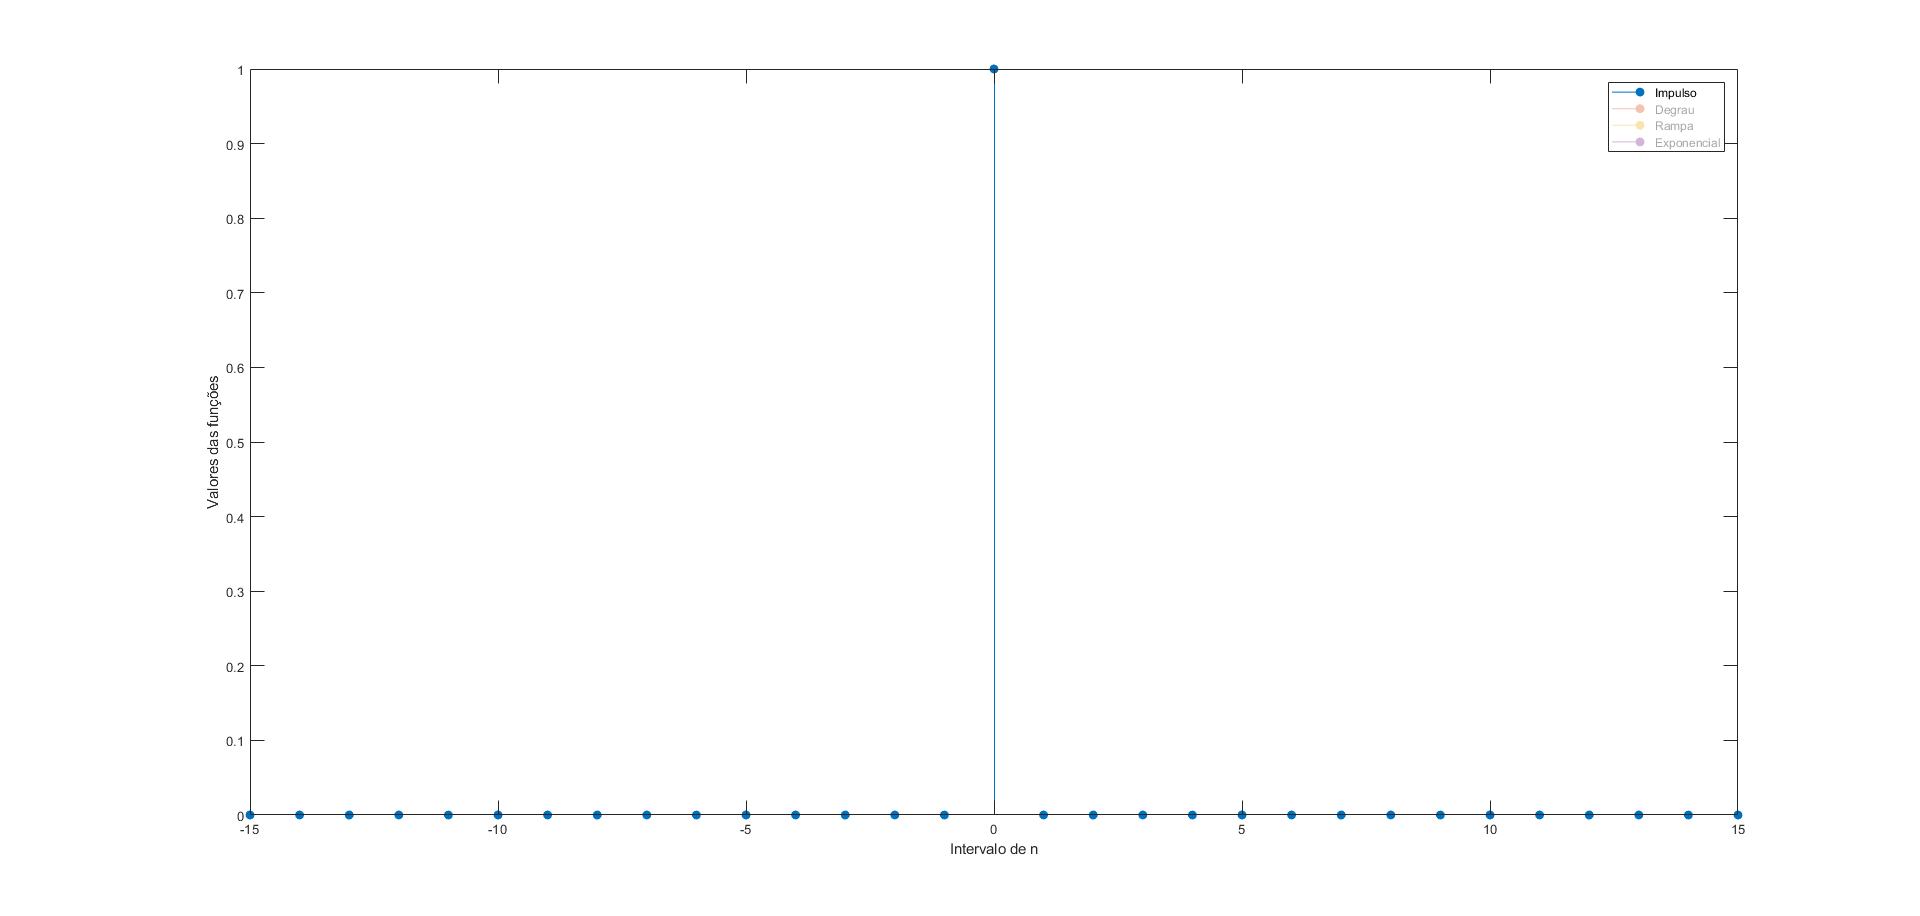
\includegraphics[width=\textwidth,scale=0.4]{1a-Imp}
				\caption{Gráfico - Impulso}
			\end{figure}
			\newpage

			\begin{figure}[!ht]
				\centering
				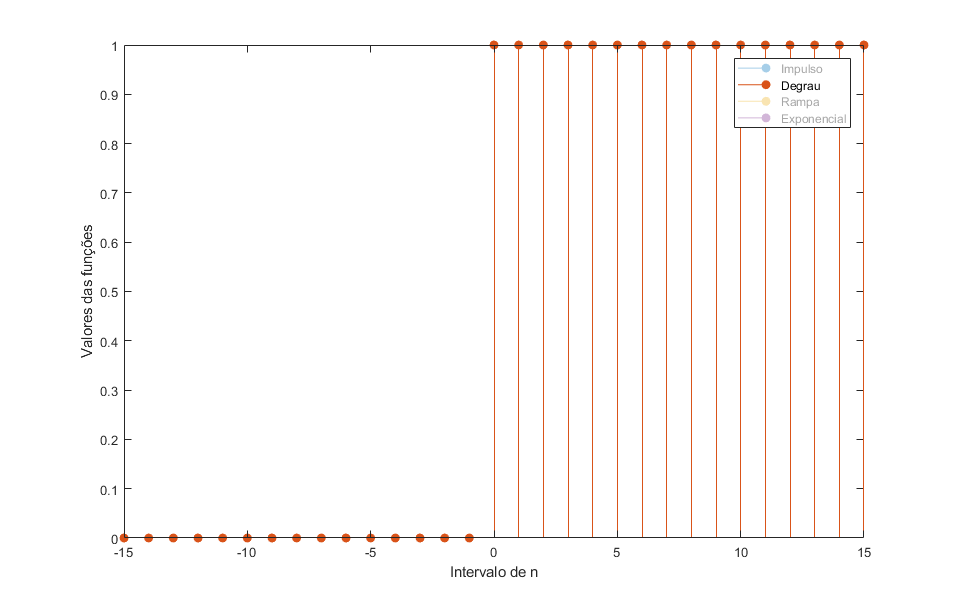
\includegraphics[scale=0.5]{1a-Deg}
				\caption{Gráfico - Degrau}
			\end{figure}

			\begin{figure}[!ht]
				\centering
				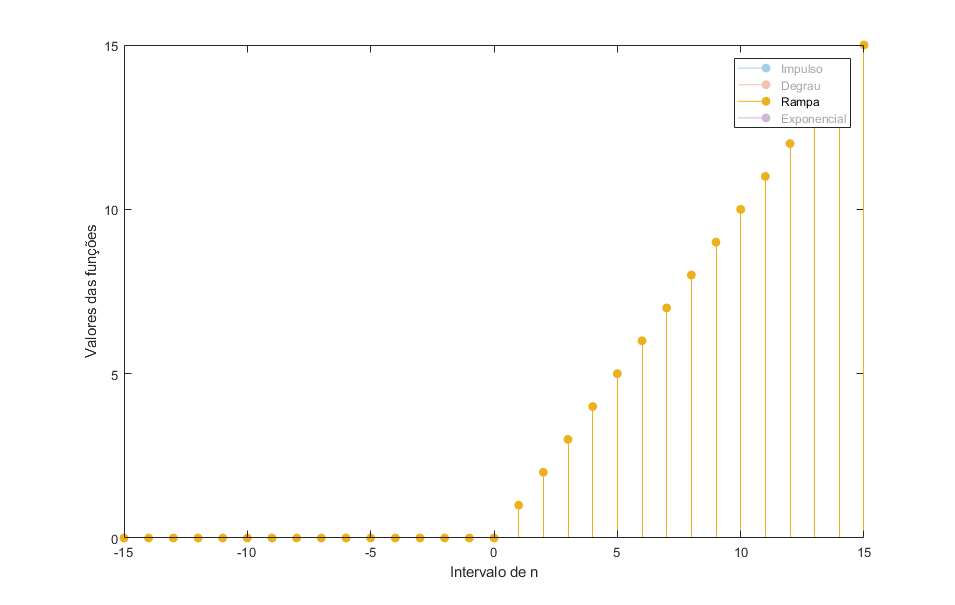
\includegraphics[scale=0.5]{1a-Ramp}
				\caption{Gráfico - Rampa}
			\end{figure}
			\newpage

			\begin{figure}[!ht]
				\centering
				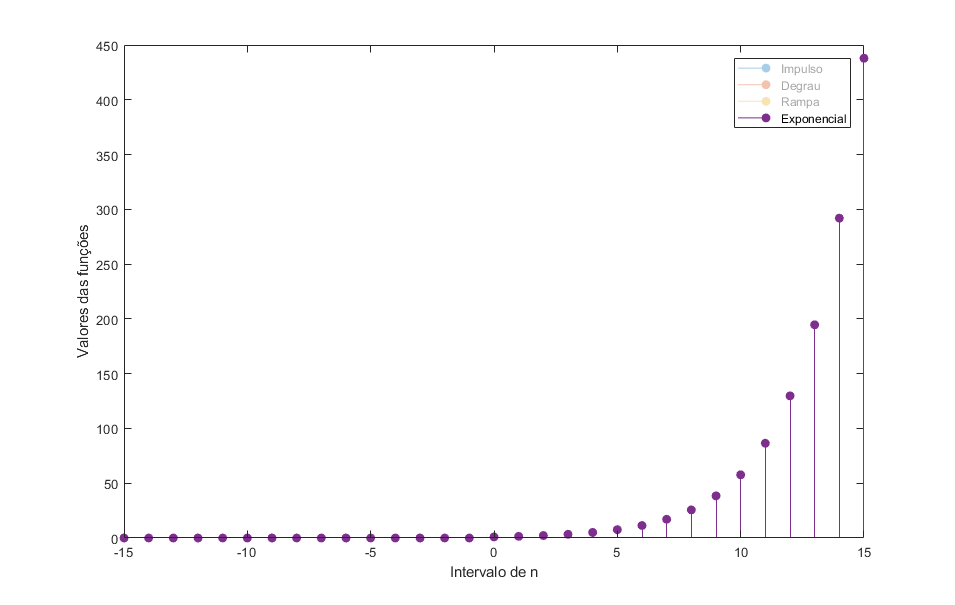
\includegraphics[scale=0.5]{1a-Exp}
				\caption{Gráfico - Exponencial}
			\end{figure}
			\newpage
	
	\subsection{Letra (B)}
	\addcontentsline{toc}{section}{Letra (B)}
	Como temos um sinal exponencial (e^a*t) | a > 1, e = 2,718 281 828 459 045 235 360 287, para t >= 2, vemos que sinal > 3. Logo, temos que ter valores de t > 1 && t < 2. Depois de tentativas experimentais, descobrimos que para t = 1.1, o valor de Pa[10] = 2.594. [insira janela grafica exponencial]
	
	\subsection{Letra (C)}
	\addcontentsline{toc}{section}{Letra (C)}
	A nossa funcao retangular (rect[n]) é formada pela subtracao de dois degraus, sendo que um deve ser deslocado da origem. No nosso exemplo, fizemos a funcao retc[n] =  u-1[k-2] - u-1[k-6], assim, obtemos um retangulo de amplitude 1 e largura M1(4). [insira essa porra de grafico aqui]
			\begin{figure}[!ht]
				\centering
				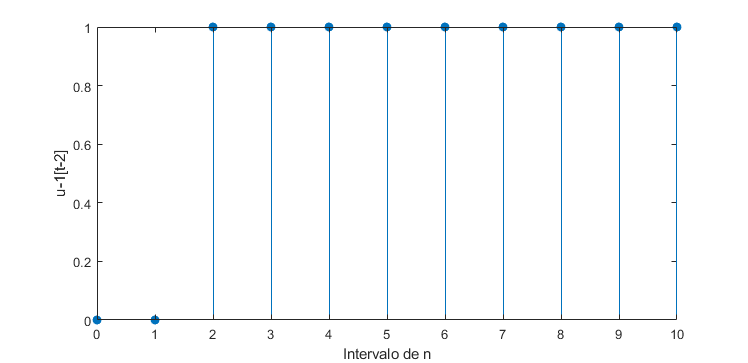
\includegraphics[scale=0.6]{1c-Deg1}
				\caption{Gráfico - Degrau}
			\end{figure}

			\begin{figure}[!ht]
				\centering
				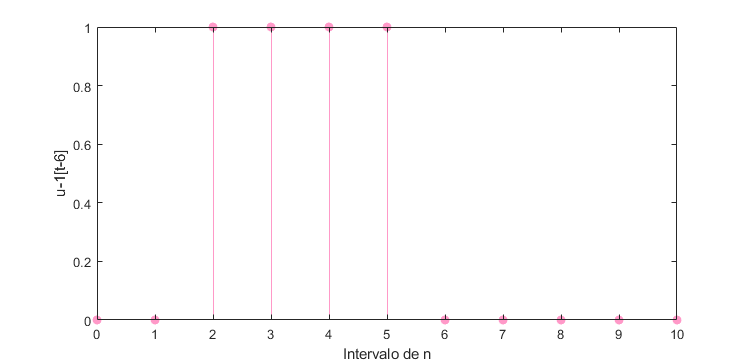
\includegraphics[scale=0.6]{1c-Deg2}
				\caption{Gráfico - Degrau}
			\end{figure}

			\begin{figure}[!ht]
				\centering
				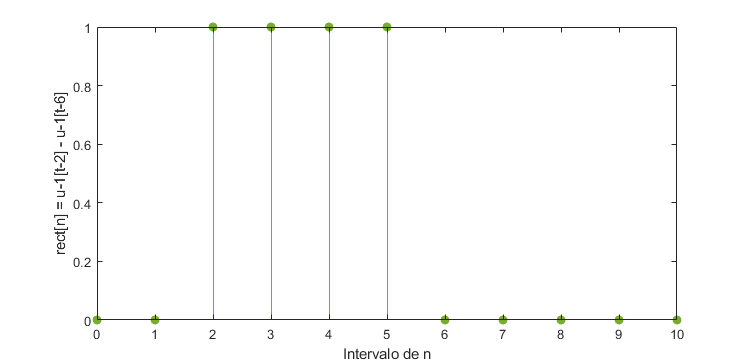
\includegraphics[scale=0.6]{1c-Rect}
				\caption{Gráfico - Rampa}
			\end{figure}
	
	\subsection{Letra (D)}
	\addcontentsline{toc}{section}{Letra (D)}
	A nossa funcao triangular (tri[n]) é formada pela subtração de duas rampas, uma rampa deslocada para esquerda 5 unidades e uma rampa de amplitude 2 centrada na origem, alem de dividir por 5 para obtermos a amplitude desejada. a funcao tri[n] = (u-2[k-5] - 2*u-2[k]) / 5. Assim, obtemos um triangulo de amplitude 1 e largura M2(5). [grafico]
	\begin{figure}[!ht]
				\centering
				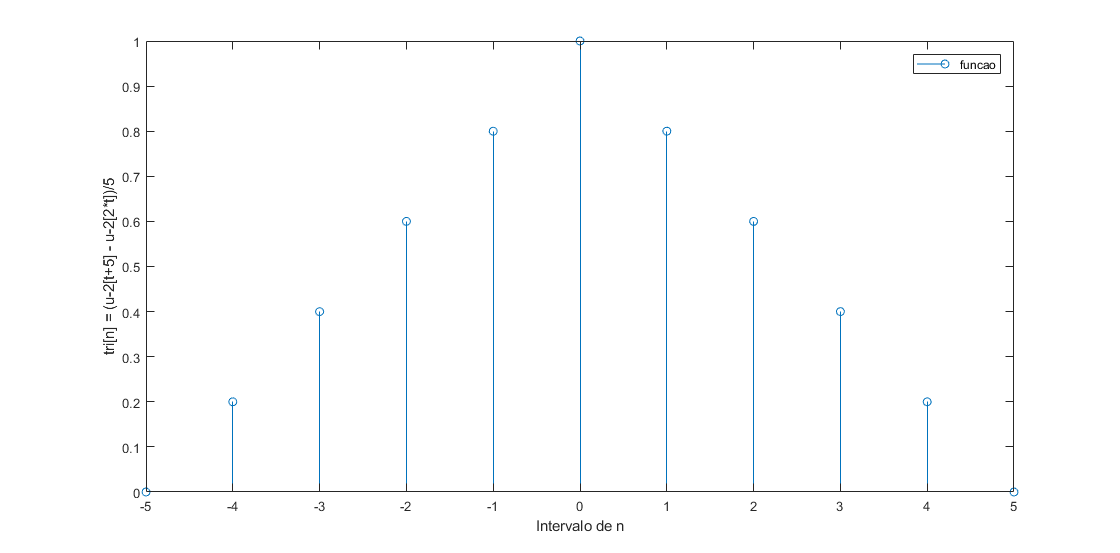
\includegraphics[scale=0.6]{1d-Tri}
				\caption{Gráfico - Degrau}
	\end{figure}


\section{Questão 2}
\addcontentsline{toc}{section}{Questão 2}
Essa questão aborda o conceito de periodicidade sobre funções. Dizemos que uma função é periódica, quando: f(k) = f(k + n*N), onde K $\in$, n $\in$ $\mathbb{Z}$, N $\in$ $\mathbb{Z}$ .
O objetivo é fazer com que o aluno coloque em prática esse conhecimento exigido por ela. Com isso, deve-se classificar as funções propostas pela questão em, periódicas ou aperiódicas, considerando o intervalo exigido.

\section{Questão 3}
\addcontentsline{toc}{section}{Questão 3}
Nessa questão podemos observar que muitos conceitos importantes estão sendo utilizados e relacionados entre si. O objetivo é obter o sinal de saída do sistemas através da convolução entre o sinal de entrada e a resposta impulsional. O primeiro fator importante abordado é de que se trata de um sistema linear invariante no tempo, ou seja, é um conjunto de operações matemáticas que não se alteram ao longo do tempo matemáticas e que só realizam operações lineares sobre os sinais de entradas afim de determinar o sinal de saída. O segundo fator é a resposta impulsional, que é saída de um sistema quando a entrada é um impulso. Por último, é a relação entre a entrada, a saída e a resposta impulsional do sistema, que por ser SLIT, podemos escrever a saída como a convolução entre o sinal de entrada e a resposta impulsional.
	\subsection{Letra (A)}
	\addcontentsline{toc}{section}{Letra (A)}
		\begin{figure}[!ht]
				\centering
				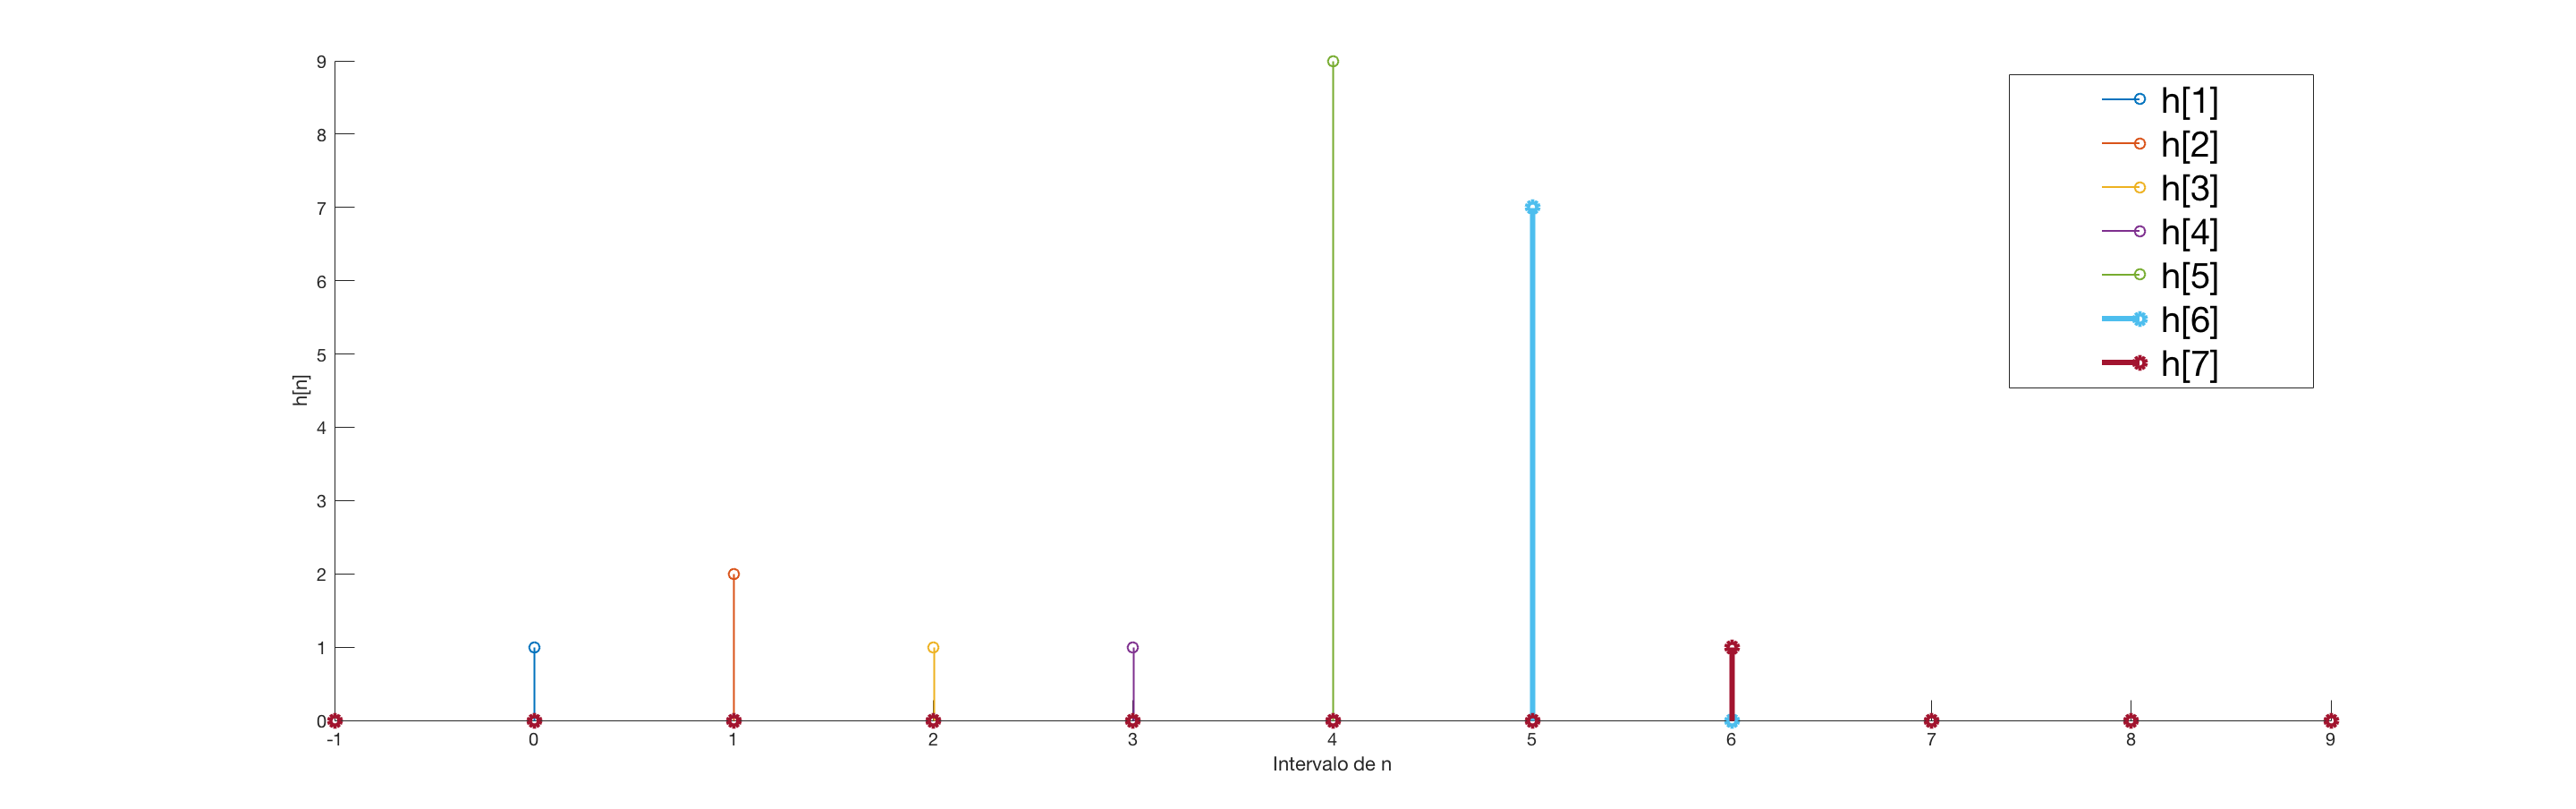
\includegraphics[width=\textwidth]{3a-respostaimpulsional}
				\caption{Gráfico - Resposta Impulsional}
		\end{figure}

\section{Questão 4}
\addcontentsline{toc}{section}{Questão 4}
Nessa questão utilizaremos os conceitos de transformada Z e equação de diferenças finitas. A transformada 
$\mathbb{Z}$ permite construir uma função a partir de uma série. Com isso, possibilitará transformar equações diferenciais finitas em equações algébricas.
Seja f(t) definida para t $\ge$ 0. A Transformada-Z da série \{f(nT)\} \text{é dada por:}
F(z) = $\mathcal{Z}\{f[n]\}$ = $\sum{_{n=0}^{\infty} f[n] z^{-n}}$

\section{Conclusão}
\addcontentsline{toc}{section}{Conclusão}

Quando necessário, os autores devem apresentar figuras, gráficos ou tabelas para apresentar os resultados obtidos e justificar suas conclusões. Todas as formas de apresentação não textual de resultados devem incluir uma legenda descrevendo em algumas palavras aquilo que está sendo representado. Essa descrição deve ser suficiente para que o leitor entenda qual a intenção dos autores na inclusão daquele item.

Gráficos, em especial, devem estar claramente anotados, incluindo indicação sobre o conteúdo dos eixos, título e legenda caso necessário. Atenção para que as figuras não se sobreponham ao texto.

Seguem alguns exemplos de gráficos e tabelas:

\section*{Índice Remissivo}
\addcontentsline{toc}{section}{Índice Remissivo}

\end{document}

